\documentclass[aspectratio=169]{beamer}
\setbeamertemplate{navigation symbols}{}
\usepackage{color,amsmath,comment, subfigure}
\usepackage{booktabs}
\usepackage{url}

%%%%%%%%%%%%%%%%%%%%%%%%%%
\title[]{Lecture 22: Network scale-up method to study groups most at-risk for HIV}
\author[]{Matthew J. Salganik}
\institute[]{Sociology 204: Social Networks\\Princeton University}
\date[]{
1/2 Network scale-up method, methods
\vfill

\begin{flushleft}
\vspace{0.6in}

\includegraphics[width=0.1\textwidth]{figures/cc.png}
\end{flushleft}
}

\begin{document}
%%%%%%%%%%%%%%%%%%%%%%%%%%%
\frame{\titlepage}
%%%%%%%%%%%%%%%%%%%%%%%%%%%
\begin{frame}

\LARGE{Network scale-up method}

\end{frame}
%%%%%%%%%%%%%%%%%%%%%%%%
\begin{frame}
\frametitle{}

\begin{center}
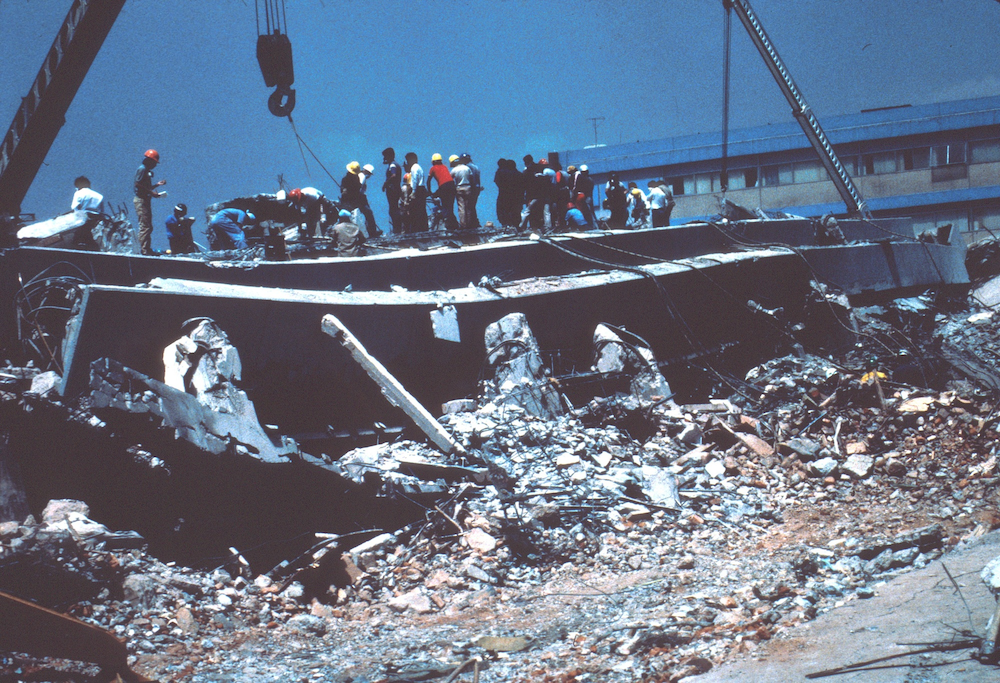
\includegraphics[width=0.8\textwidth]{figures/1985_Mexico_Earthquake_smaller.png}
\end{center}

Basic insight from Bernard et al. (1989)

\end{frame}
%%%%%%%%%%%%%%%%%
\begin{frame}

\begin{center}
\includegraphics<1>[width=0.6\textwidth]{figures/network-noedges}
\includegraphics<2>[width=0.6\textwidth]{figures/network-edges}
\includegraphics<3>[width=0.6\textwidth]{figures/network-edges-sample}
\includegraphics<4>[width=0.6\textwidth]{figures/network-edges-sample-ego}
\end{center}
\Large{
\begin{center}
\onslide<4>{$\hat{N}_H=\frac{2}{10} \times 30 = 6$}
\end{center}
}

\end{frame}
%%%%%%%%%%%%%%%%%
\begin{frame}

\begin{itemize}
\item Requires a random sample from the entire population 
\item Respondents are asked:
\begin{itemize}
\item How many people do you know who are drug injectors? 
\item How many women do you know that have given birth in the last 12 months?
\item How many people do you know who are middle school teachers?
\item $\ldots$
\item How many people do you know named Michael?
\end{itemize}
\item ``Know'' typically defined: you know them and they know you and have you been in contact with them over the past two years
\end{itemize}

\end{frame}
%%%%%%%%%%%%%%%%%
\begin{frame}

\begin{center}
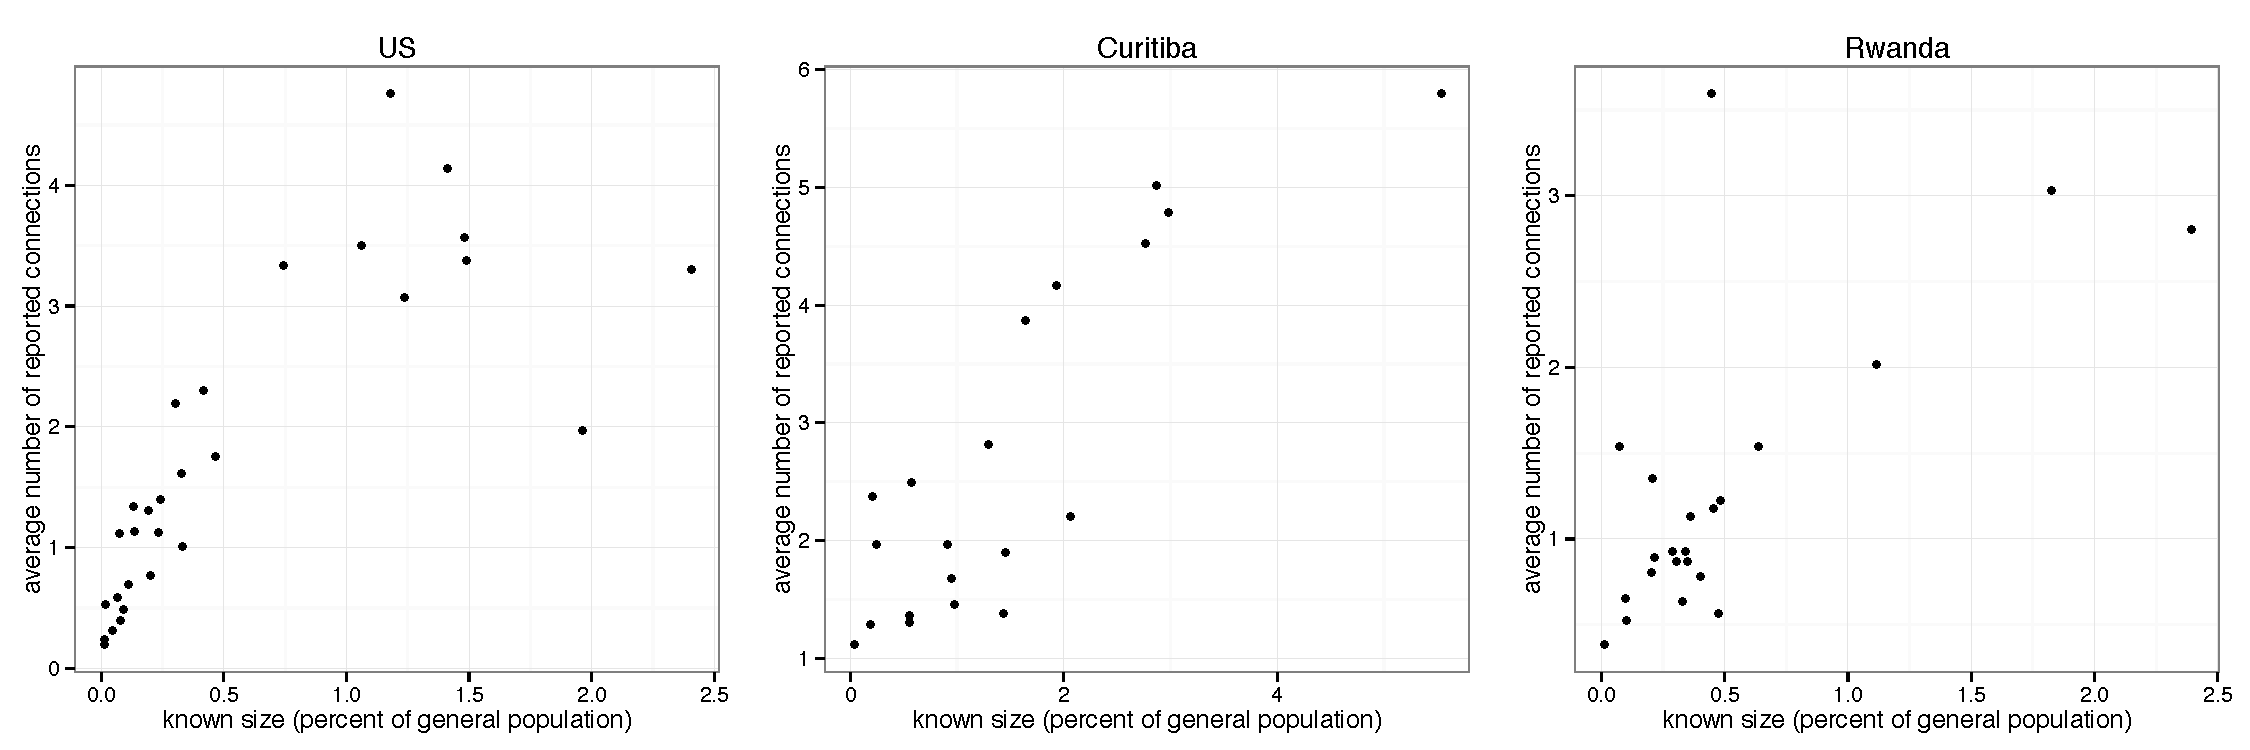
\includegraphics[width=0.95\textwidth]{figures/three_studies_truesize_known}
\end{center}
\vfill
On average, these answers are not crazy.

\end{frame}
%%%%%%%%%%%%%%%%%%
\begin{frame}

Other size estimation methods are problematic, and scale-up method has many nice properties:
\begin{itemize}
\item Requires a random sample of the general population, not specific contact with the hard-to-reach population 
\item Can be added as a module (5-10 minutes) in any existing survey 
\item Can estimate many target populations in a single survey 
\item Can be applied at the city-level, sub-national-level, or national-level
\item Statistical methods are improvable 
\item Partially self-validating because it uses groups of known size
\end{itemize}

\note{go quickly since they saw these in pre-read video}

\end{frame}
%%%%%%%%%%%%%%%%%
\begin{frame}

\begin{figure}
  \centering
   \subfigure[United States]{
     \label{fig:united_states} % Label for first subfigure
     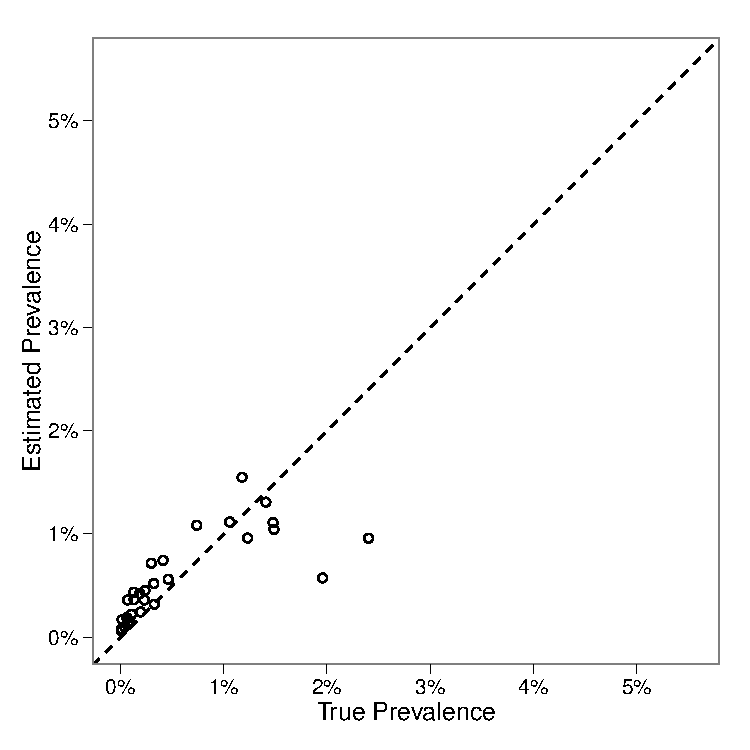
\includegraphics[width=0.3\textwidth]{figures/us-ivplot-forr01}}
  \hspace{0.0in}
    \subfigure[Curitiba]{
     \label{fig:curitiba} % Label for second subfigure
     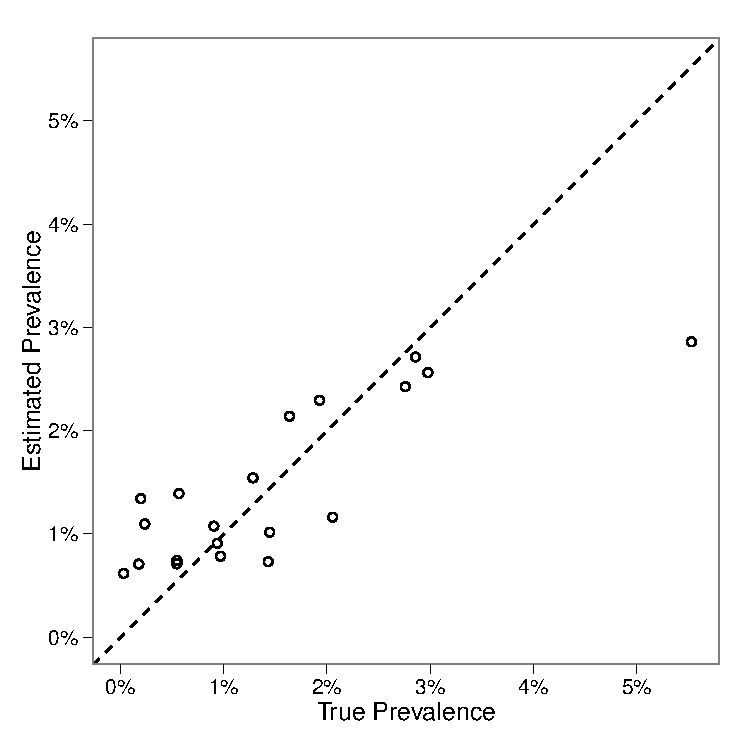
\includegraphics[width=0.3\textwidth]{figures/curitiba-ivplot-forr01}}     
  \hspace{0.0in}
    \subfigure[Rwanda]{
     \label{fig:rwanda} % Label for third subfigure
     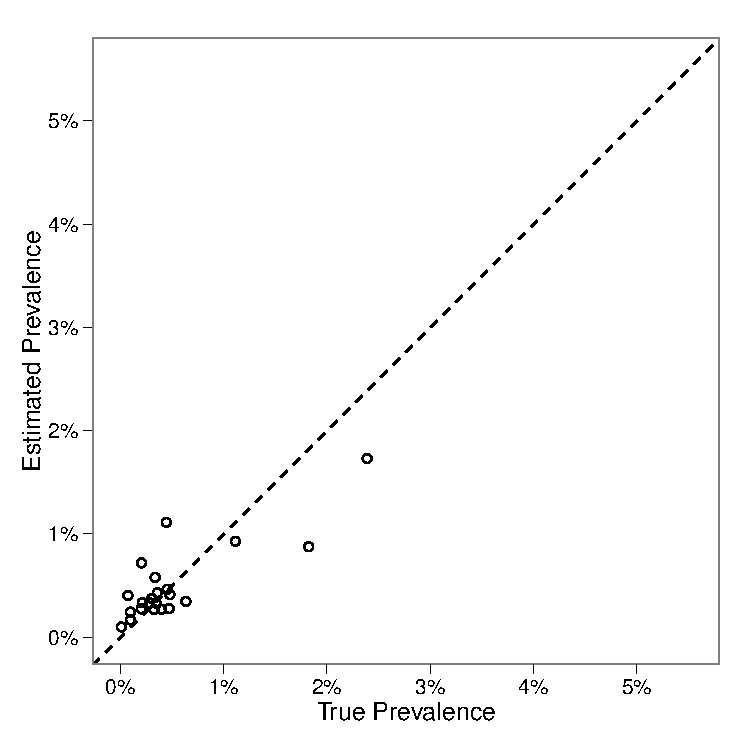
\includegraphics[width=0.3\textwidth]{figures/rwanda-ivplot-forr01}}     
\end{figure}

\end{frame}
%%%%%%%%%%%%%%%%
\begin{frame}

But, basic scale-up also has problems.  I will focus on insights about basic scale-up that we discovered from developing the generalized scale-up.

\end{frame}
%%%%%%%%%%%%%%%%%%%%%%%%%%%%%%%%%
\begin{frame}

\LARGE{Personal background}

\end{frame}
%%%%%%%%%%%%%%%%%%%%%%%%
\begin{frame}

How did I end up working on this research?\pause
\begin{itemize}
\item Working on sampling at the Census Bureau \pause
\item When I began grad school I knew about sampling and was interested in networks and Doug Heckathorn was working on respondent-driven sampling \pause
\item Respondent-driven sampling lead to the network scale-up method
\end{itemize}

\end{frame}
%%%%%%%%%%%%%%%%%%%%%%%%
\begin{frame}

\begin{columns}[t] % the "c" option specifies center vertical alignment

\column{0.45\textwidth} % column designated by a command
\begin{center}
{\Large Modeling}\\
counting with multiplicity
\end{center}

\column{0.10\textwidth}
\begin{center}
{\Large $\leftrightarrow$}
\end{center}

\column{0.40\textwidth}
\begin{center}
{\Large Empirical}\\
Rwanda (this lecture)\\
Brazil (next lecture) \\
\end{center}
\end{columns}

\end{frame}
%%%%%%%%%%%%%%%%%%%%%%%%%%%
\begin{frame}

If $\underbrace{y_{i,k} \sim Bin(d_i, N_k/N)}_\text{basic scale-up model}$, then maximum likelihood estimator is 

\begin{equation*}
\hat{N}_H = \frac{\sum_i y_{i,H}}{\sum_i \hat{d}_i} \times N
\end{equation*}
\small{
\begin{itemize}
\item $\hat{N}_H$: number of people in the hidden population
\item $y_{i,H}$: number of people in hidden population known by person $i$
\item $\hat{d}_i$: estimated number of people known by person $i$
\item $N$: number of people in the population
\end{itemize}
}
\vfill
See Killworth et al., (1998)
\end{frame}
%%%%%%%%%%%%%%%%%
\begin{frame}

\begin{center}
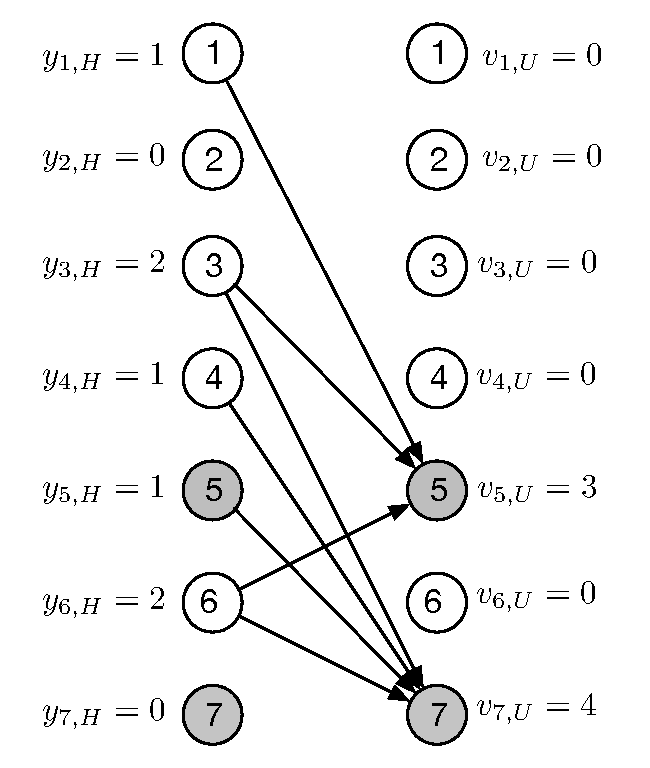
\includegraphics[height=0.8\textheight]{figures/reporting-network-panel2}
\end{center}

\end{frame}
%%%%%%%%%%%%%%%%%%
\begin{frame}

\begin{equation*}
\mbox{total out-reports} = \mbox{total in-reports}
\end{equation*}

\pause

\begin{align}
\mbox{total out-reports} & = \mbox{size of hidden pop}  \times  \nonumber \\ & \qquad \mbox{in-reports per member of hidden pop}  \nonumber
\end{align}

\pause 

\begin{equation*}
\mbox{size of hidden pop} = \frac{ \mbox{total out-reports} } { \mbox{in-reports per member of hidden pop} }
\end{equation*}

\end{frame}
%%%%%%%%%%%%%%%%%
\begin{frame}

\only<1>{
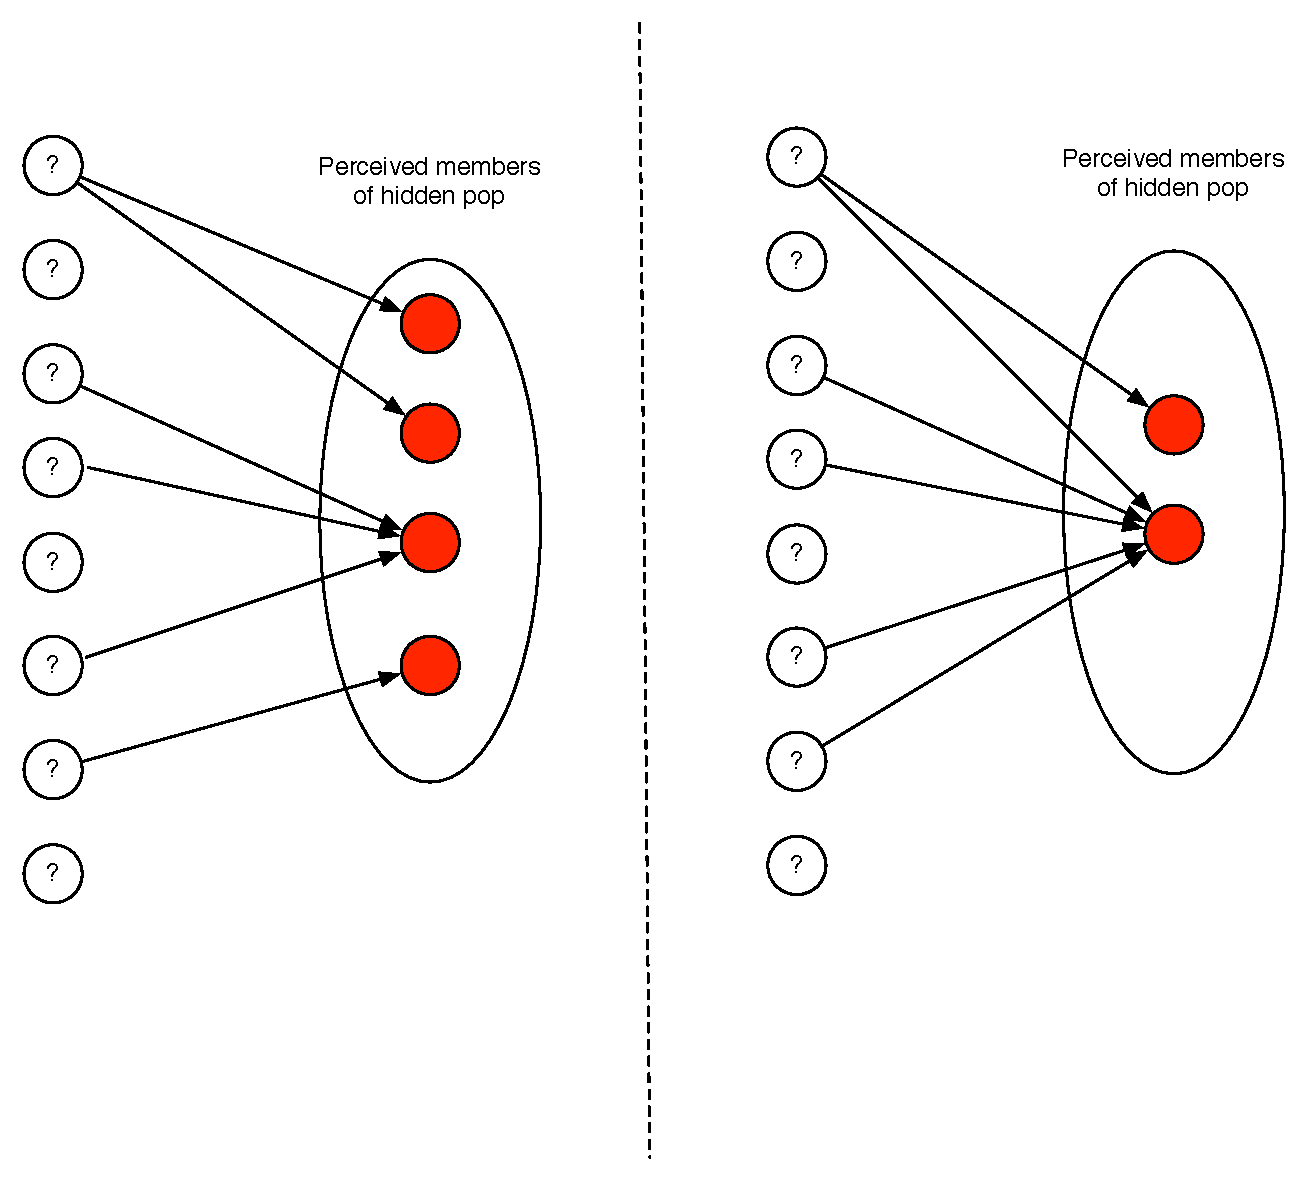
\includegraphics[width=0.8\textwidth]{figures/identification_problem_all}
}
\only<2>{
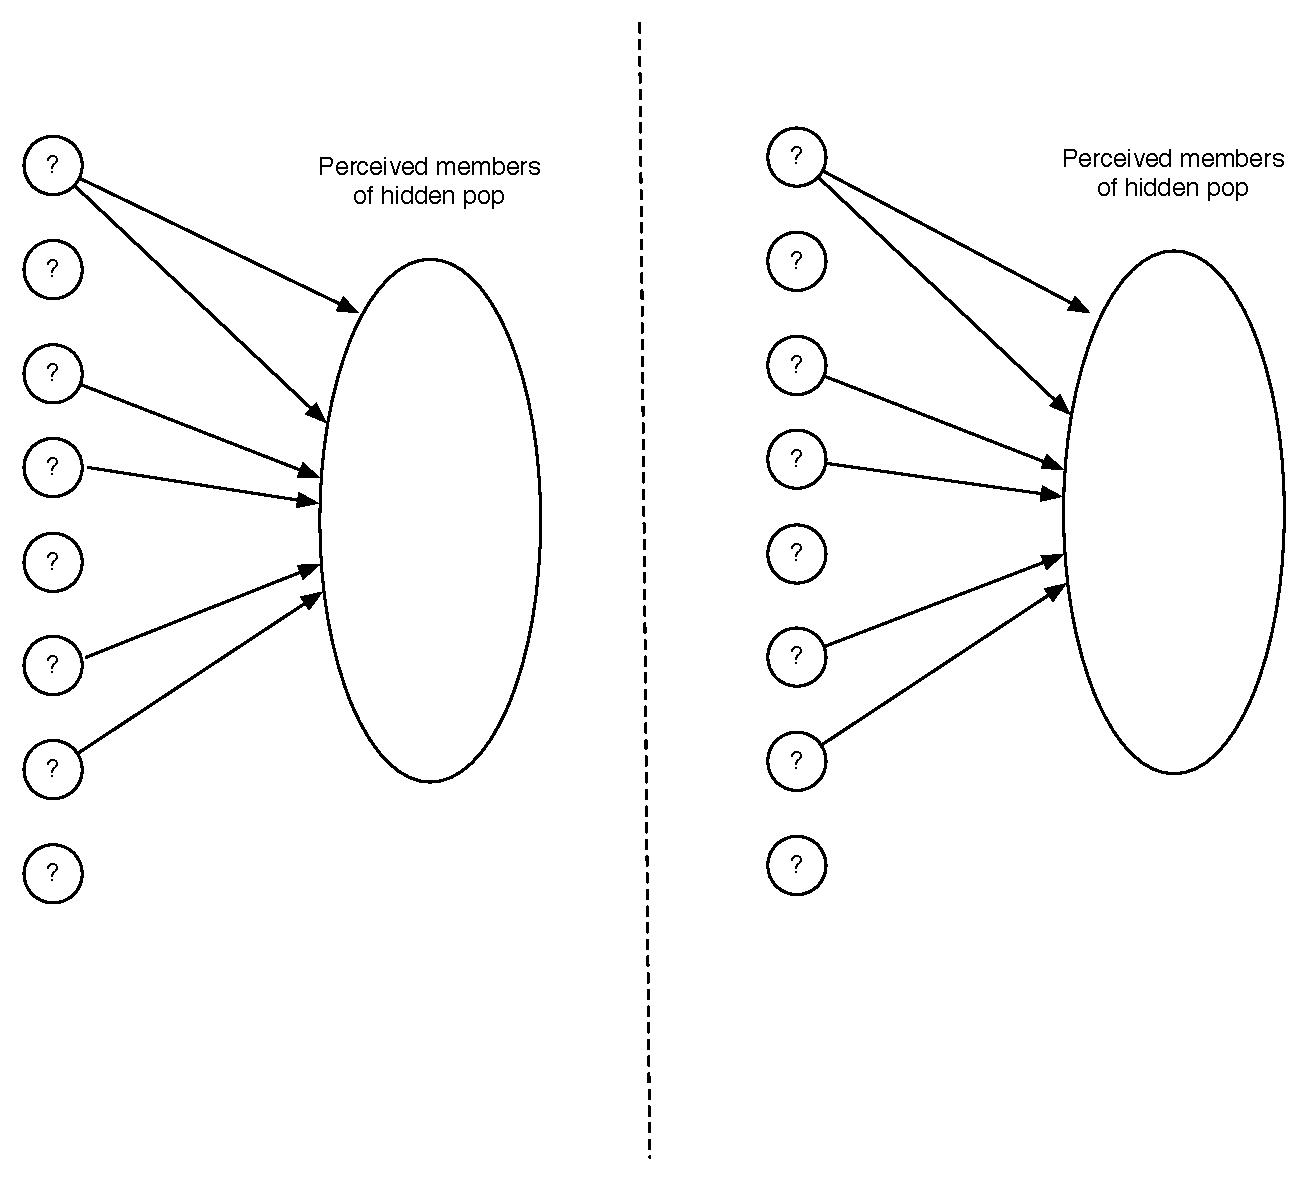
\includegraphics[width=0.8\textwidth]{figures/identification_problem_partial}
}
\end{frame}
%%%%%%%%%%%%%%%%%%
\begin{frame}

\begin{equation*}
\underbrace{N_H}_{\text{size of hidden pop}} = \frac{ \overbrace{ \sum_{i \in F} y_{i,H} }^{\text{total out-reports}} } { \underbrace{ \left( \sum_{i \in U} v_{i,F} / N_H \right) }_{\text{in-reports per member of hidden pop}} }
\end{equation*}
\pause
\vfill
If there are no false positives,
\begin{equation*}
\underbrace{N_H}_{\text{size of hidden pop}} = \frac{ \overbrace{ \sum_{i \in F} y_{i,H} }^{\text{total out-reports}} } { \underbrace{ \left( \sum_{\textcolor{blue}{i \in H}} v_{i,F} / N_H \right) }_{\text{avg visible degree of hidden pop}} }
\end{equation*}

\end{frame}
%%%%%%%%%%%%%%%%%
\begin{frame}

Generalized scale-up identity
\begin{equation*}
\underbrace{N_H}_{\text{size of hidden pop}} = \frac{ \overbrace{ \sum_{i \in F} y_{i,H} }^{\text{total out-reports}} } { \underbrace{ \left( \sum_{\textcolor{blue}{i \in H}} v_{i,F} / N_H \right) }_{\text{avg visible degree of hidden pop}} }
\end{equation*}

\vfill
Basic scale-up estimator
\only<1>{
\begin{equation*}
\hat{N}_H = \frac{\sum_{i \in s_F} y_{i,H}}{\sum_{i \in s_F} \hat{d}_i} \times N
\end{equation*}
}

\only<2>{
\begin{equation*}
\underbrace{\hat{N}_H}_{\text{est size of hidden pop}} = \frac{\overbrace{\sum_{i \in s_F} y_{i,H}}^\text{total out-reports}} {\underbrace{\sum_{i \in s_F} \hat{d}_{i, U} / N}_\text{avg degree of pop} }
\end{equation*}
}

\end{frame}
%%%%%%%%%%%%%%%%%%
\begin{frame}

Counting with multiplicity approach:
\begin{itemize}
\item no assumptions about the underlying social network
\item extends naturally to incomplete social awareness
\item extends naturally to incomplete frames
\item extends naturally to complex sample designs
\end{itemize}

\end{frame}
%%%%%%%%%%%%%%%%%%%%%%%%%%%
\begin{frame}

\begin{center}
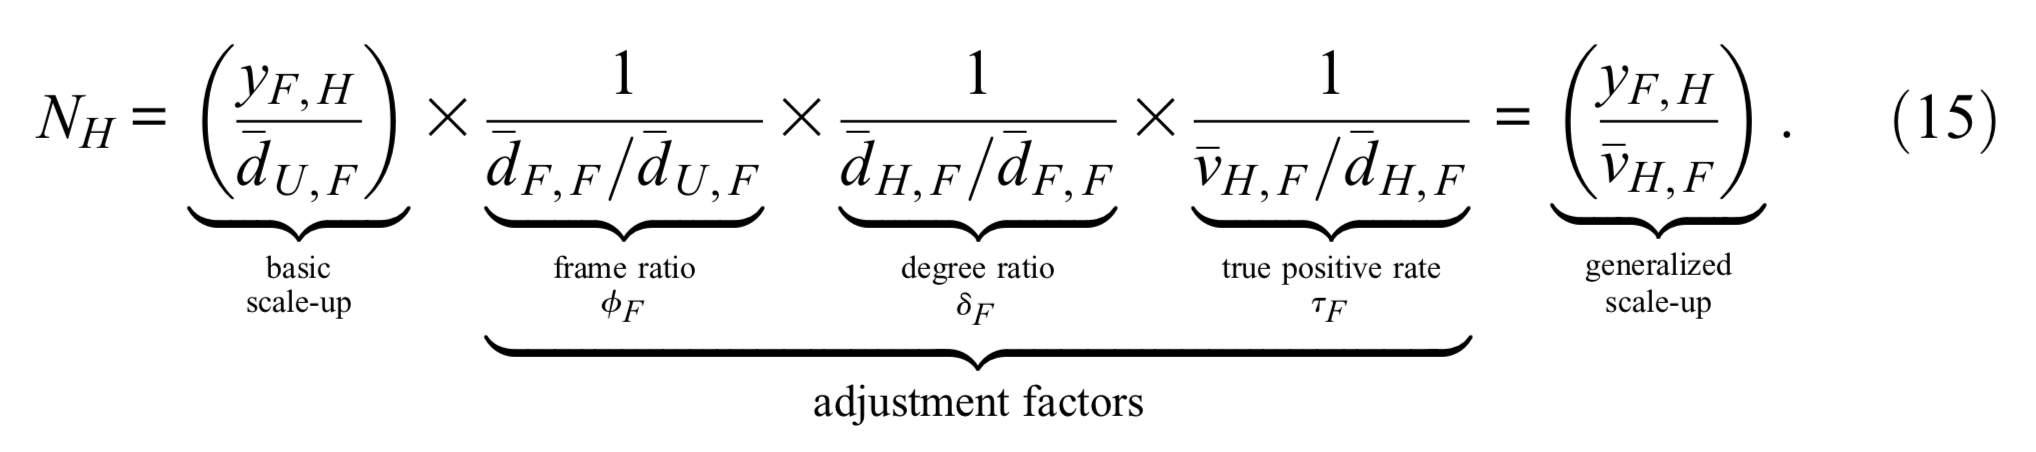
\includegraphics[width=0.95\textwidth]{figures/feehan_generalizing_2016_eq15}
\end{center}

\end{frame}
%%%%%%%%%%%%%%%%%%%%%%%%%%%%%
\begin{frame}

Frame ratio: Less a focus for us.  As a first approximation, sampling frame is adults you don't want to include kids in any of the reports

\end{frame}
%%%%%%%%%%%%%%%%%%%%%%%%%%%%
\begin{frame}

Degree ratio: If the hidden population has smaller network sizes than the general population, the size of the hidden population will be underestimated.  Likewise, if the hidden population has larger network sizes than the general population, the size of the hidden population will be overestimated.

\end{frame}
%%%%%%%%%%%%%%%%%%%%%%%%%%%%
\begin{frame}

Set of egos can be different from set of alters.
\vfill
\begin{columns}[c]
\column{0.3\textwidth}
\framebox{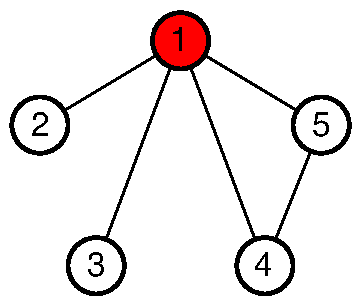
\includegraphics[height=0.8in]{figures/folded_network_slides}}
\phantom{1234}$p=0.2$
\column{0.6\textwidth}
\pause
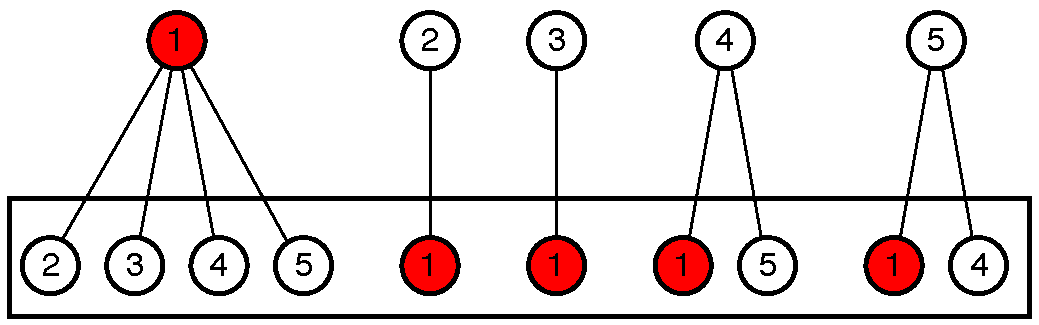
\includegraphics[height=0.8in]{figures/unfolded_network_slides}
\phantom{123456789123456789101112}
\phantom{1234567891234}$p_{alter}=0.4$
\end{columns}
\vfill
\pause
\begin{equation*}
p_{alter}=p \times \frac{\mbox{avg. degree (hidden pop.)}}{\mbox{avg. degree (general pop.)}}=p \delta
\end{equation*}
\vfill
Estimates will be biased by a factor of $\delta_F$ (``degree ratio'')

\end{frame}
%%%%%%%%%%%%%%%%%%
\begin{frame}

True positive rate: If people are connected to people in the hidden population but not aware of it, the size of the hidden population will be underestimated 

\end{frame}
%%%%%%%%%%%%%%%%%%%%%%%%%%%%
\begin{frame}

How might imperfect knowledge impact scale-up estimates?\\
Ego is not aware of everything about all of their alters.
\begin{center}
\includegraphics<1>[width=0.7\textwidth]{figures/network-edges-sample-ego-noinfotxerror}
\includegraphics<2>[width=0.7\textwidth]{figures/network-edges-sample-ego-infotxerror-formatt}
\end{center}
\pause
\vfill
Estimates will be biased by a factor of $\tau_F$ (``true positive rate'')

\vfill
More about this in next lecture 

\end{frame}
%%%%%%%%%%%%%%%%%%
\begin{frame}

\begin{center}
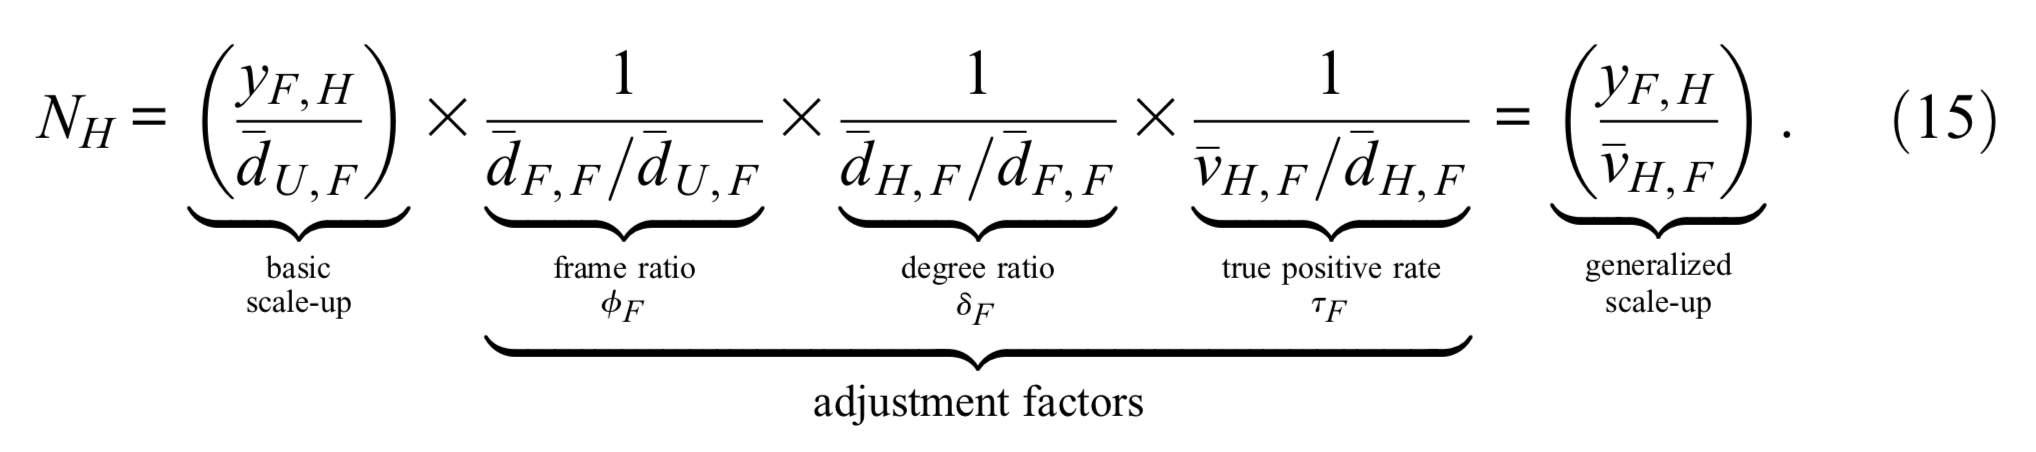
\includegraphics[width=0.95\textwidth]{figures/feehan_generalizing_2016_eq15}
\end{center}
 
\end{frame}
%%%%%%%%%%%%%%%%%%%%%%%%
\begin{frame}
\frametitle{From a talk I gave at a UNAIDS workshop}

Generalized scale-up approach
\begin{itemize}
\item simple estimators (just addition, subtraction, multiplication, and division)
\item handles incomplete social awareness
\item no assumptions about the underlying social network
\item handles incomplete frames
\item handles complex sample designs
\end{itemize}

\vfill
and could still be very wrong in practice!

\end{frame}
%%%%%%%%%%%%%%%%%%%%%%%%%
\begin{frame}

\begin{center}
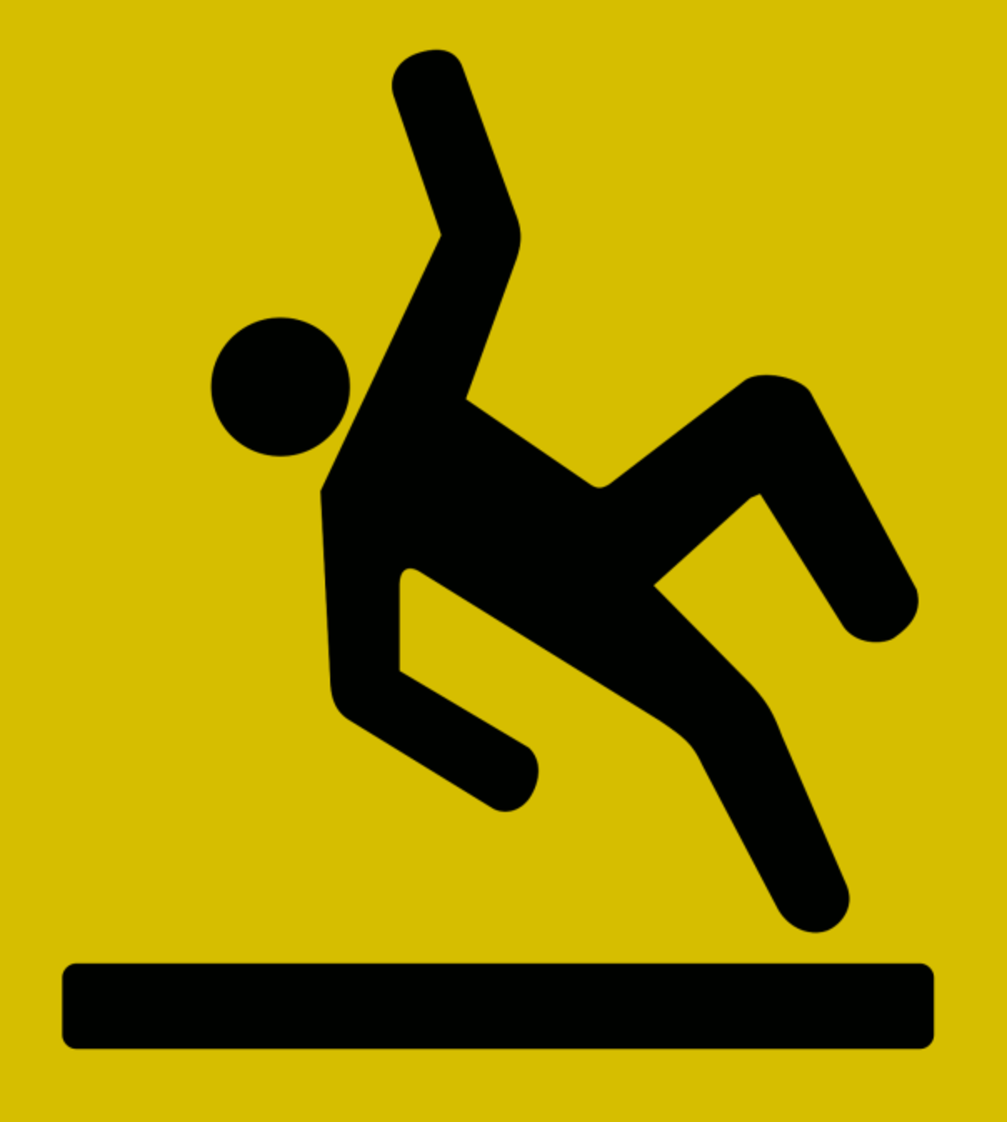
\includegraphics[width=0.5\textwidth]{figures/slippery-when-wet}
\end{center}

\end{frame}
%%%%%%%%%%%%
\begin{frame}

Assumptions can be put into four broad categories
\begin{itemize}
\item sampling
\item social network structure
\item reporting
\item survey construction
\end{itemize}

\end{frame}
%%%%%%%%%%%
\begin{frame}

Results for non-sampling assumptions have this form:
\begin{center}
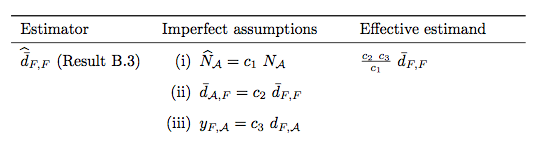
\includegraphics[width=0.7\textwidth]{figures/feehan_estimating_2014_tabd1_result1}
\end{center}

\end{frame}
%%%%%%%%%%%%
\begin{frame}

\begin{center}
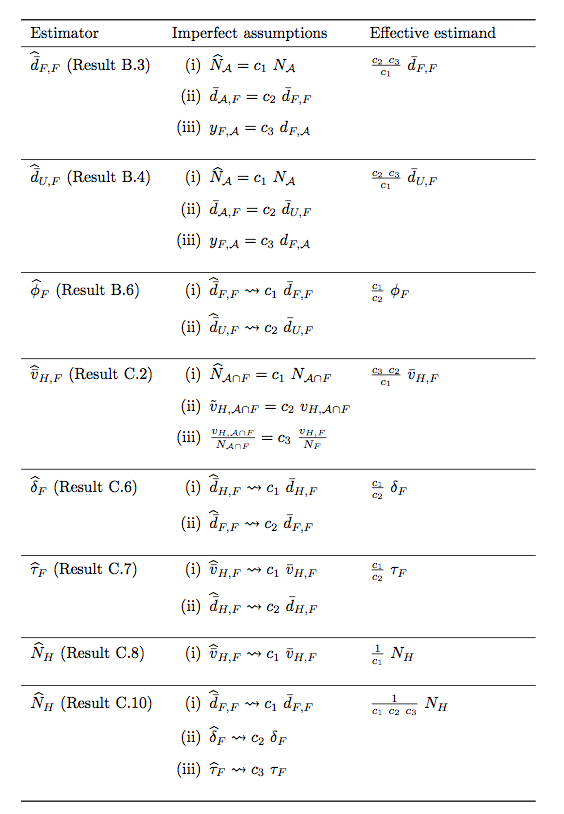
\includegraphics[height=\textheight]{figures/feehan_estimating_2014_tabd1}
\end{center}

\end{frame}
%%%%%%%%%%%%%
\begin{frame}

\begin{center}
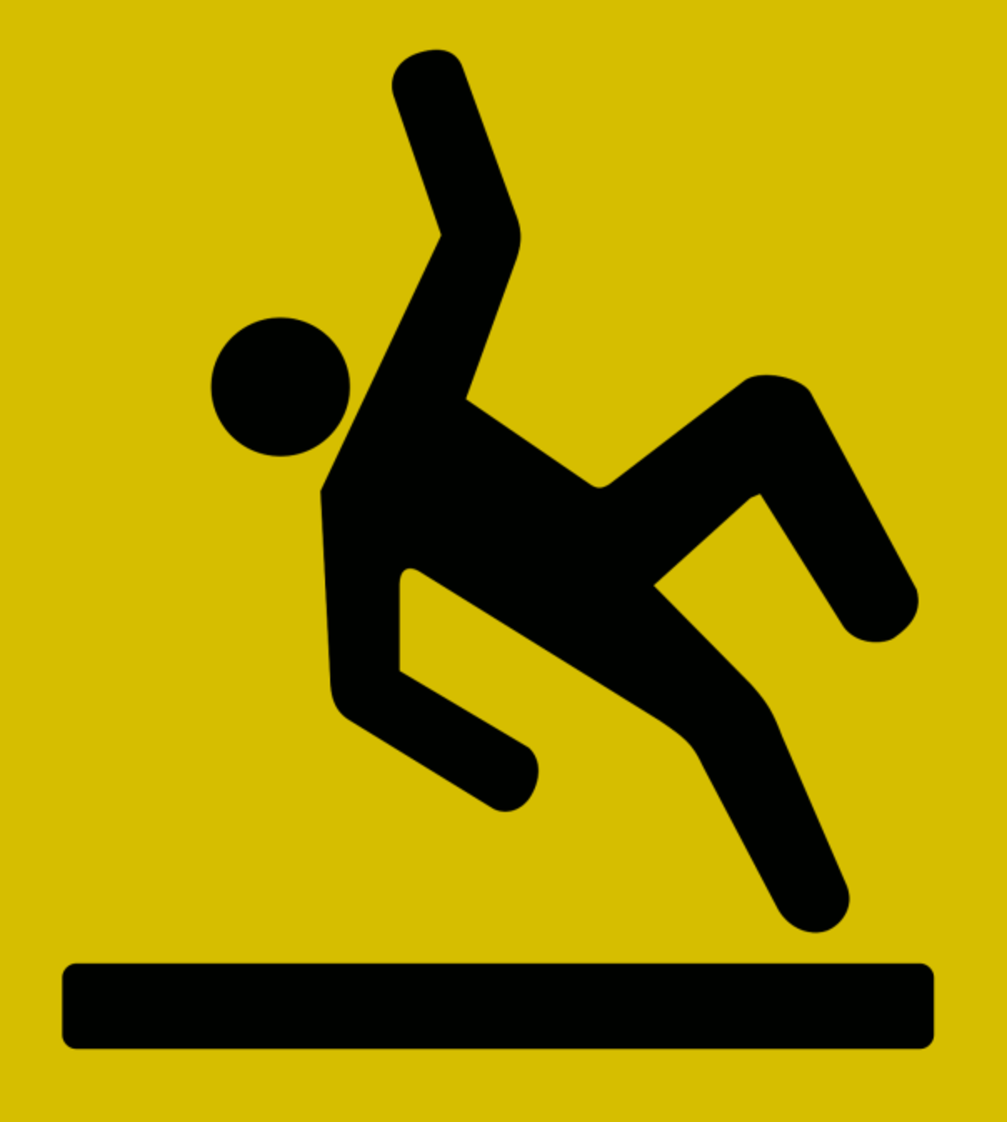
\includegraphics[width=0.3\textwidth]{figures/slippery-when-wet}
\end{center}

Fails when:
\begin{itemize}
\item adjustment factors not measured
\item adjustment factors measured poorly
\item reporting not consistent with awareness
\item variance estimation fails
\item  . . . .
\end{itemize}

\end{frame}
%%%%%%%%%%%%%%%%%%%%%%%%%%%%%%%
\begin{frame}

\begin{columns}[t] % the "c" option specifies center vertical alignment

\column{0.45\textwidth} % column designated by a command
\begin{center}
{\Large Modeling}\\
counting with multiplicity
\end{center}

\column{0.10\textwidth}
\begin{center}
{\Large $\leftrightarrow$}
\end{center}

\column{0.40\textwidth}
\begin{center}
{\Large Empirical}\\
Rwanda (this lecture)\\
Brazil (next lecture) \\
\end{center}
\end{columns}

\end{frame}

\end{document}
